\chapter{\index{Access Security}Access Security}

\section{Overview}

This chapter describes access security. i.e. the system that limits access to IOC databases. It consists of the following 
sections:

\begin{enumerate}\item Overview - This section

\item Quick start - A summary of the steps necessary to start access security.

\item User's Guide - This explains what access security is and how to use it.

\item Design Summary - Functional Requirements and Design Overview.

\item Application Programmer's Interface

\item Database Access Security - Access Security features for EPICS IOC databases.

\item Channel Access Security - Access Security features in Channel Access

\item Trapping Channel Access Writes - This allows trapping of all writes from external channel access clients.

\item Implementation Overview

\end{enumerate}The requirements for access security were generated at ANL/APS in 1992. The requirements document is:

EPICS: Channel Access Security - Functional Requirements, Ned D. Arnold, 03/-9/92.

This document is available through the EPICS website.

\section{Quick Start}

In order to ``turn on" access security for a particular IOC the following must be done:

\begin{itemize}\item Create the access security file.

\item IOC databases may have to be modified

\begin{itemize}

\item Record instances may have to have values assigned to field ASG. If ASG is null the record is in group 
DEFAULT. 

\item Access security files can be reloaded after iocInit via a subroutine record with \verb|asSubInit| and 
\verb|asSubProcess| as the associated subroutines. Writing the value 1 to this record will cause a reload.

\end {itemize}

\item The startup script must contain the following command before iocInit.

\verb|asSetFilename("/full/path/to/accessSecurityFile")|

\item The following is an optional command.

\verb|asSetSubstitutions("var1=sub1,var2=sub2,..."))|

\end{itemize}

The following rules decide if access security is turned on for an IOC:

\begin{itemize}

\item If asSetFilename is not executed before iocInit, access security will NEVER be started..

\item If asSetFile is given and any error occurs while first initializing access security, then ALL access to that ioc is 
denied.

\item If after successfully starting access security, an attempt is made to restart and an error occurs then the previous 
access security configuration is maintained.

\end{itemize}

After an IOC has been booted with access security enabled, the access security rules can be changed by issuing the 
asSetFilename, asSetSubstitutions, and asInit. The functions asInitialize, asInitFile, and asInitFP, which are described 
below, can also be used.

\section{User's Guide}

\subsection{Features}

Access security protects IOC databases from unauthorized Channel Access Clients. Access security is based on the 
following:

\begin{itemize}\item Who:  Userid of the channel access client.

\item Where:  Hostid where the user is logged on. This is the host on which the channel access client exists. Thus no 
attempt is made to see if a user is local or is remotely logged on to the host.

\item What:  Individual fields of records are protected. Each record has a field containing the Access Security Group 
(ASG) to which the record belongs. Each field has an access security level, which must be 0 or 1.The security level 
is defined in the ascii record definition file. Thus the access security level for a field is the same for all record 
instances of a record type.

\item When:  Access rules can contain input links and calculations similar to the calculation record. 

\end{itemize}\subsection{Limitations}

An IOC database can be accessed only via Channel Access or via the vxWorks or ioc shell. It is assumed that access to the 
local IOC console is protected via physical security and \verb|telnet|/\verb|rlogin| access protected via normal networking and 
physical security methods.

No attempt has been made to protect against the sophisticated saboteur. Network security methods must be used to limit 
access to the subnet on which the iocs reside.

\subsection{Definitions}

This document uses the following terms:

\begin{itemize}\item \index{ASL}ASL:  Access Security Level (Called access level in Req Doc)

\item \index{ASG}ASG:  Access Security Group (Called PV Group in Req Doc)

\item \index{UAG}UAG:  User Access Group

\item \index{HAG}HAG:  Host Access Group

\end{itemize}\subsection{Access Security Configuration File}

\index{Access Security: Configuration File}This section describes the format of a file containing definitions of the user access groups, host access groups, and access 
security groups. An IOC creates an access configuration database by reading an access configuration file (the extension 
.\verb|acf| is recommended). Lets first give a simple example and then a complete description of the syntax.

\subsubsection{Simple Example}

\begin{verbatim}
UAG(uag) {user1,user2}
HAG(hag) {host1,host2}
ASG(DEFAULT) {
    RULE(1,READ)
    RULE(1,WRITE) {
        UAG(uag)
        HAG(hag)
    }
}
\end{verbatim}These rules provide read access to anyone located anywhere and write access to \verb|user1| and \verb|user2| if they are located at 
\verb|host1| or \verb|host2|.

\begin{verbatim}
\end{verbatim}\subsubsection{Syntax Definition}

In the following description:

\begin{description}\item \verb|[ ]|Surrounds optional elements

\verb||\verb+|+\verb||Separates alternatives

\verb|...|Means that an arbitrary number of definitions may be given.

\end{description}Any line beginning with a \verb|#| character is a comment

The elements \textless{}name\textgreater{}, \textless{}user\textgreater{}, \textless{}host\textgreater{}, \textless{}pvname\textgreater{}, and \textless{}calculation\textgreater{} can be given a quoted or unquoted strings. The 
rules for unquoted strings are the same as for database definitions.



\begin{verbatim}UAG(<name>) [{ <user> [, <user> ...] }]
...
HAG(<name>) [{ <host> [, <host> ...] }]
...
ASG(<name>) [{
    [INP<index>(<pvname>)
    ...]
    RULE(<level>,NONE | READ | WRITE [, NOTRAPWRITE | TRAPWRITE]) {
        [UAG(<name> [,<name> ...])]
        [HAG(<name> [,<name> ...])]
        CALC(<calculation>)
    }
    ...
}]
...
\end{verbatim}\index{NOTRAPWRITE}
\index{TRAPWRITE}\subsubsection{Discussion}

\begin{itemize}\item \index{UAG}UAG:  User Access Group. This is a list of user names. The list may be empty. The same user can appear in 
multiple UAGs. For vxWorks iocs the user name is taken from the user field of the boot parameters.

\item \index{HAG}HAG: Host Access Group. This is a list of host names. It may be empty. The same host name can appear in 
multiple HAGs. For iocs the host name is taken from the target name of the boot parameters. NOTE: host names 
are converted to lower case.

\item \index{ASG - access security configuration}ASG: An access security group. The group ``\verb|DEFAULT|" is a special case. If a member specifies a null group or a 
group which has no ASG definition then the member is assigned to the group ``\verb|DEFAULT|".

\item \index{INP - access security configuration}INP\textless{}index\textgreater{}  Index must have one of the values ``\verb|A|" to ``\verb|L|". These are just like the \verb|INP| fields of a 
calculation record. It is necessary to define \verb|INP| fields if a \verb|CALC| field is defined in any \verb|RULE| for the ASG.

\item \index{RULE}RULE   This defines access permissions. \textless{}\verb|level|\textgreater{} must be 0 or 1. Permission for a level 1 field implies 
permission for level 0 fields. The permissions are \verb|NONE|, \verb|READ|, and \verb|WRITE|. \verb|WRITE| permission implies 
\verb|READ| permission. The standard EPICS record types have all fields set to level 1 except for \verb|VAL|, \verb|CMD| 
(command), and \verb|RES| (reset). An optional argument specifies if writes should be trapped. See the section 
below on trapping Channel Access writes for how this is used. If not given the default is NOTRAPWRITE.

\begin{itemize}

\item \index{UAG}UAG specifies a list of user access groups that can have the access privilege. If UAG is not defined 
then all users are allowed.

\item \index{HAG}HAG specifies a list of host access groups that have the access privilege. If HAG is not defined then 
all hosts are allowed.

\item \index{CALC - access security configuration}CALC is just like the \verb|CALC| field of a calculation record except that the result must evaluate to TRUE 
or \verb|FALSE|. The rule only applies if the calculation result is \verb|TRUE|, where the actual test for \verb|TRUE| is 
\verb|(0.99 < result < 1.01)|. Anything else is regarded as \verb|FALSE| and will cause the rule to be 
ignored. Assignment statements are not permitted in CALC expressions here.

\end{itemize}
\end{itemize}

Each IOC record contains a field \verb|ASG|, which specifies the name of the ASG to which the record belongs. If this field is 
null or specifies a group which is not defined in the access security file then the record is placed in group ``\verb|DEFAULT|".

The access privilege for a channel access client is determined as follows:

\begin{enumerate}\item The ASG associated with the record is searched.

\item Each RULE is checked for the following:

\begin{enumerate}

\item The field's level must be less than or equal to the level for this RULE.

\item If UAG is defined, the user must belong to one of the specified UAGs. If UAG is not defined all users are 
accepted.

\item If HAG is defined, the user's host must belong to one one of the HAGs. If HAG is not defined all hosts are 
accepted.

\item If CALC is specified, the calculation must yield the value 1, i.e. TRUE. If any of the INP fields associated 
with this calculation are in INVALID alarm severity the calculation is considered false. The actual test for 
TRUE is .99 \textless{} result \textless{} 1.01.

\end{enumerate}

\item The maximum access allowed by step 2 is the access chosen.

\end{enumerate}

Multiple RULEs can be defined for a given ASG, even RULEs with identical levels and access permission.

\subsection{ascheck - Check Syntax of Access Configuration File}

After creating or modifying an access configuration file it can be checked for syntax errors by issuing the command:

\begin{verbatim}ascheck -S "xxx=yyy,..." < "filename"
\end{verbatim}\index{ascheck}This is a Unix command. It displays errors on \verb|stdout|. If no errors are detected it prints nothing. Only syntax errors not 
logic errors are detected. Thus it is still possible to get your self in trouble. The flag \verb|-S |means a set of macro 
substitutions may appear. This is just like the macro substitutions for dbLoadDatabase.

\subsection{IOC Access Security Initialization}

\index{Access Security: Initialization}In order to have access security turned on during IOC initialization the following command must appear in the startup file 
before \verb|iocInit| is called:

\begin{verbatim}asSetFilename("/full/path/to/access/security/file.acf")
\end{verbatim}\index{asSetFilename}If this command is not used then access security will not be started by \verb|iocInit|. If an error occurs when iocInit calls 
\verb|asInit| than all access to the ioc is disabled, i.e. no channel access client will be able to access the ioc. Note that this 
command does not read the file itself, it just saves the argument string for use later on, nor does it save the current 
working directory, which is why the use of an absolute path-name for the file is recommended (a path name could be 
specified relative to the current directory at the time when \verb|iocInit| is run, but this is not recommended if the IOC also 
loads the subroutine record support as a later reload of the file might happen after the current directory had been changed).

Access security also supports macro substitution just like \verb|dbLoadDatabase|. The following command specifies the 
desired substitutions:

\begin{verbatim}asSetSubstitutions("var1=sub1,var2=sub2,...")
\end{verbatim}\index{asSetSubstitutions}This command must be issued before \verb|iocInit|.

After an IOC is initialized the access security database can be changed. The preferred way is via the subroutine record 
described in the next section. It can also be changed by issuing the following command to the vxWorks shell:

\begin{verbatim}asInit
\end{verbatim}\index{asInit}It is also possible to reissue \verb|asSetFilename| and/or \verb|asSetSubstitutions |before \verb|asInit|. If any error occurs 
during \verb|asInit| the old access security configuration is maintained. It is NOT permissable to call \verb|asInit| before 
\verb|iocInit| is called. 

Restarting access security after ioc initialization is an expensive operation and should not be used as a regular procedure.

\subsection{Database Configuration}



\subsubsection{Access Security Group}

\index{Access Security Group}Each database record has a field \verb|ASG| which holds a character string. Any database configuration tool can be used to give 
a value to this field. If the ASG of a record is not defined or is not equal to a ASG in the configuration file then the record 
is placed in \verb|DEFAULT|. 

\subsubsection{Subroutine Record Support}

Two subroutines, which can be attached to a subroutine record, are available (provided with \verb|iocCore|):

\begin{verbatim}asSubInit
asSubProcess
\end{verbatim}\index{asSubInit}
\index{asSubProcess}NOTE: These subroutines are automatically registered thus do NOT put a \verb|registrar| definition in your database 
definition file.

If a record is created that attaches to these routines, it can be used to force the IOC to load a new access configuration 
database. To change the access configuration:

\begin{enumerate}\item Modify the file specified by the last call to \verb|asSetFilename| so that it contains the new configuration desired.

\item Write a 1 to the subroutine record \verb|VAL| field. Note that this can be done via channel access.

\end{enumerate}The following action is taken:

\begin{enumerate}\item When the value is found to be 1, \verb|asInit| is called and the value set back to 0.

\item The record is treated as an asynchronous record. Completion occurs when the new access configuration has been 
initialized or a time-out occurs. If initialization fails the record is placed into alarm with a severity determined by 
\verb|BRSV|.

\end{enumerate}\subsubsection{Record Type Description}

Each field of each record type has an associated access security level of \verb|ASL0| or \verb|ASL1|. See the chapter ``Database 
Definition" for details.

\subsection{Example:}

Lets design a set of rules for a Linac. Assume the following:

\begin{enumerate}\item Anyone can have read access to all fields at anytime.

\item Linac engineers, located in the injection control or control room, can have write access to most level 0 fields only if 
the Linac is not in operational mode.

\item Operators, located in the injection control or control room, can have write access to most level 0 fields anytime.

\item The operations supervisor, linac supervisor, and the application developers can have write access to all fields but 
must have some way of not changing something inadvertently.

\item Most records use the above rules but a few (high voltage power supplies, etc.) are placed under tighter control. 
These will follow rules 1 and 4 but not 2 or 3.

\item IOC channel access clients always have level 1 write privilege.

\end{enumerate}Most Linac IOC records will not have the \verb|ASG| field defined and will thus be placed in ASG ``\verb|DEFAULT|". The following 
records will have an \verb|ASG| defined:

\begin{itemize}\item \verb|LI:OPSTATE| and any other records that need tighter control have \verb|ASG|="\verb|critical|". One such record could be 
a subroutine record used to cause a new access configuration file to be loaded. \verb|LI_OPSTATE |has the value (0,1) 
if the Linac is (not operational, operational).

\item \verb|LI:lev1permit |has \verb|ASG|="\verb|permit|". In order for the \verb|opSup|, \verb|linacSup|, or an \verb|appDev| to have write 
privilege to everything this record must be set to the value 1.

\end{itemize}The following access configuration satisfies the above rules.

\begin{verbatim}UAG(op) {op1,op2,superguy}
UAG(opSup) {superguy}
UAG(linac) {waw,nassiri,grelick,berg,fuja,gsm}
UAG(linacSup) {gsm}
UAG(appDev) {nda,kko}
HAG(icr) {silver,phebos,gaea}
HAG(cr) {mars,hera,gold}
HAG(ioc) {ioclic1,ioclic2,ioclid1,ioclid2,ioclid3,ioclid4,ioclid5}
ASG(DEFAULT) {
    INPA(LI:OPSTATE)
    INPB(LI:lev1permit)
    RULE(0,WRITE) {
        UAG(op)
        HAG(icr,cr)
        CALC("A=1")
    }
    RULE(0,WRITE) {
        UAG(op,linac,appdev)
        HAG(icr,cr)
        CALC("A=0")
    }
    RULE(1,WRITE) {
        UAG(opSup,linacSup,appdev)
        CALC("B=1")
    }
    RULE(1,READ)
    RULE(1,WRITE) {
        HAG(ioc)
    }
}
ASG(permit) {
    RULE(0,WRITE) {
        UAG(opSup,linacSup,appDev)
    }
    RULE(1,READ)
    RULE(1,WRITE) {
        HAG(ioc)
    }
}
ASG(critical) {
    INPB(LI:lev1permit)
    RULE(1,WRITE) {
        UAG(opSup,linacSup,appdev)
        CALC("B=1")
    }
    RULE(1,READ)
    RULE(1,WRITE) {
        HAG(ioc)
    }
}
\end{verbatim}\section{Design Summary}

\subsection{Summary of Functional Requirements}

A brief summary of the Functional Requirements is:

\begin{enumerate}\item Each field of each record type is assigned an access security level.

\item Each record instance is assigned to a unique access security group.

\item Each user is assigned to one or more user access groups.

\item Each node is assigned to a host access group.

\item For each access security group a set of access rules can be defined. Each rule specifies: 

\begin{enumerate}

\item Access security level

\item READ or READ/WRITE access.

\item An optional list of User Access Groups or * meaning anyone.

\item An optional list of Host Access Groups or * meaning anywhere.

\item Conditions based on values of process variables

\end{enumerate}

\end{enumerate}

\subsection{Additional Requirements}

\subsubsection{Performance}

Although the functional requirements doesn't mention it, a fundamental goal is performance. The design provides almost 
no overhead during normal database access and moderate overhead for the following: channel access client/server 
connection, ioc initialization, a change in value of a process variable referenced by an access calculation, and dynamically 
changing a records access control group. Dynamically changing the user access groups, host access groups, or the rules, 
however, can be a time consuming operation. This is done, however, by a low priority IOC task and thus does not impact 
normal ioc operation. 

\subsubsection{Generic Implementation}

Access security should be implemented as a stand alone system, i.e. it should not be imbedded tightly in database or 
channel access.

\subsubsection{No Access Security within an IOC}

Within an IOC no access security is invoked. This means that database links and local channel access clients calls are not 
subject to access control. Also test routines such as dbgf should not be subject to access control.

\subsubsection{Defaults}

It must be possible to easily define default access rules.

\subsubsection{Access Security is Optional}

When an IOC is initialized, access security is optional.

\subsection{Design Overview}

The implementation provides a library of routines for accessing the security system. This library has no knowledge of 
channel access or IOC databases, i.e. it is generic. Database access, which is responsible for protecting an IOC database, 
calls library routines to add each IOC record to one of the access control groups.

Lets briefly discuss the access security system and how database access and channel access interact with it.

\subsubsection{Configuration File}

User access groups, host access groups, and access security groups are configured via an ASCII file.

\subsubsection{Access Security Library}

The access security library consists of the following groups of routines: initialization, group manipulation, client 
manipulation, access computation, and diagnostic. The initialization routine reads a configuration file and creates a 
memory resident access control database. The group manipulation routines allow members to be added and removed from 
access groups. The client routines provide services for clients attached to members.

\subsubsection{IOC Database Access Security}

The interface between an IOC database and the access security system.

\subsubsection{Channel Access Security}

Whenever the Channel Access broadcast server receives a \verb|ca_search| request and finds the process variable, it calls 
\verb|asAddClient|.  Whenever it disconnects it calls \verb|asRemoveClient|. Whenever it issues a get or put to the database it 
must call \verb|asCheckGet| or \verb|asCheckPut|.

\subsection{Comments}

It is likely that the access rules will be defined such that many IOCs will attach to a common process variable. As a result 
the IOC containing the PV will have many CA clients.

What about password protection and encryption? I maintain that this is a problem to be solved in a level above the access 
security described in this document. This is the issue of protecting against the sophisticated saboteur.

\subsection{Performance and Memory Requirements}

Performance has not yet been measured but during the tests to measure memory usage no noticeable change in 
performance during ioc initialization or during Channel Access clients connection was noticed. Unless access privilege is 
violated the overhead during channel access gets and puts is only an extra comparison.

In order to measure memory usage, the following test was performed:

\begin{enumerate}\item A database consisting of 5000 soft analog records was created.

\item A channel access client (\verb|caput|) was created that performs \verb|ca_put|s on each of the 5000 channels. Each time it 
begins a new set of puts the value increments by 1.

\item A channel access client (\verb|caget|) was created that has monitors on each of the 5000 channels.

\end{enumerate}The memory consumption was measured before \verb|iocInit|, after \verb|iocInit|, after \verb|caput| connected to all channels, and 
after \verb|caget| connected to all 5000 channels. This was done for APS release 3.11.5 (before access security) and the first 
version which included access security. The results were:
\begin{center}\begin{longtable}{p{1.0in}p{1.0in}p{1.0in}}
\textbf{} & \textbf{R3.11.5} & \textbf{After}\\
\hline
Before iocInit & 4,244,520 & 4,860,840\\
After iocInit & 4,995,416 & 5,964,904\\
After caput & 5,449,780 & 6,658,868\\
After caget & 8,372,444 & 9,751,796
\end{longtable}\end{center}


Before the database was loaded the memory used was 1,249,692 bytes. Thus most of the memory usage before iocInit 
resulted from storage for records. The increase since R3.11.5 results from added fields to \verb|dbCommon|. Fields were added 
for access security, synchronous time support and for the new caching put support. The other increases in memory usage 
result from the control blocks needed to support access control. The entire design was based on maximum performance. 
This resulted in increased memory usage.

\section{Access Security Application Programmer's Interface}

\subsection{Introduction}

File \verb|asLib.h |describes the access security data structures and the last section of this chapter has a diagram describing 
the relationship between the structures. The structures are:

\begin{itemize}\item ASBASE - Contains the list head for lists of UAGs, HAGs, and ASGs

\item UAG - A user access group.

\item HAG - A host access group

\item ASG - An access secuity group. It contains the list head for ASGINPs, ASGRULEs, and ASGMEMBERs

\item ASGINP - Contains the information for an INPx.

\item ASGRULE - Contains the information for a rule

\item ASGMEMBER - Contains the information for a member of an access secururity group. It contains the list head for 
ASGCLIENTs.

\end{itemize}All structures except ASGMEMBER and ASGCLIENT are created by the access security library itself  when it reads an 
access security file. An ASGMEMBER is created each time asAddMember is called by code that interfaces to the 
database. An ASGCLIENT is created each time asAddClient is called by a channel access server.

\subsection{Definitions}

The following are descriptions of arguments of routines described later.

\begin{verbatim}typedef struct asgMember *ASMEMBERPVT;
typedef struct asgClient *ASCLIENTPVT;
typedef int (*ASINPUTFUNCPTR)(char *buf,int max_size);
typedef enum{
    asClientCOAR   /*Change of access rights*/
    /*For now this is all*/
} asClientStatus;
typedef void (*ASCLIENTCALLBACK)(ASCLIENTPVT,asClientStatus);

\end{verbatim}\subsection{Initialization}

\begin{verbatim}long asInitialize(ASINPUTFUNPTR inputFunction)
long asInitFile(const char *filename,const char *substitutions)
long asInitFP(FILE *fp,const char *substitutions)
\end{verbatim}\index{asInitialize}
\index{asInitFile}
\index{asInitFP}These routines read an access definition file and perform all initialization necessary. The caller must provide a routine to 
provide input lines for \verb|asInitialize. asInitFile |and \verb|asInitFP |do their own input and also perform macro 
substitutions.

The initilization routines can be called multiple times. If an access system already exists the old definitions are removed 
and the new one initialized. Existing members are placed in the new \verb|ASG|s. 

\subsection{Group manipulation}

The routines are called by code that knows how to associate ASG names with the database. In the case of IOC databases, 
dbCommon has a field ASG. At IOC initialization a call is made to asAddMember for every record instance in the IOC 
database.

\subsubsection{add Member}

\begin{verbatim}long asAddMember(ASMEMBERPVT *ppvt, const char *asgName);
\end{verbatim}\index{asAddMember}This routine adds a new member to ASG \verb|asgName|. The calling routine must provide storage for \verb|ASMEMBERPVT|. Upon 
successful return *\verb|ppvt| will be equal to the address of storage used by the access control system. The access system 
keeps an orphan list for all \verb|asgNames| not defined in the access configuration.

The caller must provide permanent storage for \verb|asgName|.

This routine returns \verb|S_asLib_asNotActive| without doing anything if access control is not active.

\subsubsection{remove Member}

\begin{verbatim}long asRemoveMember(ASMEMBERPVT *ppvt);
\end{verbatim}\index{asRemoveMember}This routine removes a member from an access control group. If any clients are still present it returns an error status of 
S\_asLib\_clientExists without removing the member.

This routine returns S\_asLib\_asNotActive without doing anything if access control is not active.

\subsubsection{get Member Pvt}

\begin{verbatim}void *asGetMemberPvt(ASMEMBERPVT pvt);
\end{verbatim}\index{asGetMemberPvt}For each member, the access system keeps a pointer that can be used by the caller. This routine returns the value of the 
pointer.

This routine returns NULL if access security is not active 

\subsubsection{put Member Pvt}

\begin{verbatim}long asPutMemberPvt(ASMEMBERPVT pvt,void *userPvt);
\end{verbatim}\index{asPutMemberPvt}This routine is used to set the pointer returned by asGetMemberPvt.

This routine returns \verb|S_asLib_asNotActive| without doing anything if access control is not active.

\subsubsection{change Group}

\begin{verbatim}long asChangeGroup(ASMEMBERPVT *ppvt,const char *newAsgName);
\end{verbatim}\index{asChangeGroup}This routine changes the group for an existing member. The access rights of all clients of the member are recomputed.

The caller must provide permanent storage for \verb|newAsgName|.

This routine returns \verb|S_asLib_asNotActive| without doing anything if access control is not active.

\subsection{ Client Manipulation}

This code is called by a channel access server.

\subsubsection{add Client}

\begin{verbatim}long asAddClient(ASCLIENTPVT *ppvt,ASMEMBERPVT pvt,int asl,
                       const char *user,char*host);
\end{verbatim}\index{asAddClient}This routine adds a client to an ASG member. The calling routine must provide storage for \verb|ASCLIENTPVT|. 
\verb|ASMEMBERPVT| is the value that was set by calling \verb|asAddMember|. The database code and the server code must develop 
a convention that allows the server code to locate the \verb|ASMEMBERPVT.| For IOC databases,  \verb|ASMEMBERPVT| is kept in 
dbCommon\verb|. asl| is the access security level.

The caller must provide permanent storage for \verb|user| and \verb|host|. Note that user is ``const char *" but host is just ``char *". 
The reason is the host names are converted to lower case.

This routine returns \verb|S_asLib_asNotActive| without doing anything if access control is not active.

\subsubsection{change Client}

\begin{verbatim}long asChangeClient(ASCLIENTPVT ppvt,int asl,

const char *user,char*host);
\end{verbatim}\index{asChangeClient}This routine changes one or more of the values \verb|asl|, \verb|user|, and \verb|host| for an existing client. Again the caller must provide 
permanent storage for \verb|user| and \verb|host|. It is permissible to use the same \verb|user| and \verb|host| used in the call to 
\verb|asAddClient| with different values.

This routine returns \verb|S_asLib_asNotActive| without doing anything if access control is not active.

\subsubsection{remove Client}

\begin{verbatim}long asRemoveClient(ASCLIENTPVT *pvt);
\end{verbatim}\index{asRemoveClient}This call removes a client.

This routine returns \verb|S_asLib_asNotActive| without doing anything if access control is not active.

\subsubsection{get Client Pvt}

\begin{verbatim}void *asGetClientPvt(ASCLIENTPVT pvt); 
\end{verbatim}\index{asGetClientPvt}For each client, the access system keeps a pointer that can be used by the caller. This routine returns the value of the 
pointer.

This routine returns \verb|NULL| if access security is not active. 

\subsubsection{put Client Pvt}

\begin{verbatim}void asPutClientPvt(ASCLIENTPVT pvt, void *userPvt); 
\end{verbatim}\index{asPutClientPvt}This routine is used to set the pointer returned by \verb|asGetClientPvt|.

\subsubsection{register Callback}

\begin{verbatim}long asRegisterClientCallback(ASCLIENTPVT pvt,

ASCLIENTCALLBACK pcallback);
\end{verbatim}\index{asRegisterClientCallback} This routine registers a callback that will be called whenever the access privilege of the client changes.

This routine returns \verb|S_asLib_asNotActive| without doing anything if access control is not active.

\subsubsection{check Get}

\begin{verbatim}long asCheckGet(ASCLIENTPVT pvt); 
\end{verbatim}\index{asCheckGet(}This routine, actually a macro, returns (\verb|TRUE|,\verb|FALSE|) if the client (has, doesn't have) get access rights.

\subsubsection{check Put}

\begin{verbatim}long asCheckPut(ASCLIENTPVT pvt);
\end{verbatim}\index{asCheckPut}This routine, actually a macro, returns (\verb|TRUE|,\verb|FALSE|) if the client (has, doesn't have) put access rights.

\subsubsection{asTrapWriteBefore and asTrapWriteAfter}

\index{asTrapWriteBefore}
\index{asTrapWriteAfter}\begin{verbatim}void *asTrapWriteBefore(ASCLIENTPVT clientPvt,
const char *userid, const char *hostid, void *serverSpecific);
void *asTrapWriteAfter(void *trapPvt);
\end{verbatim}These routines must be called before and after any write performed for a client. The value returned by 
\verb|asTrapWriteBefore| must be the value passed to \verb|asTrapWriteAfter|. The severSpecific argument is assigned to 
the \verb|serverSpecific| field of the \verb|asTrapWriteMessage| described below. 

\subsection{Access Computation}

\subsubsection{compute all Asg}

\begin{verbatim}long asComputeAllAsg(void); 
\end{verbatim}\index{asComputeAllAsg}This routine calls \verb|asComputeAsg| for each access security group.

This routine returns \verb|S_asLib_asNotActive| without doing anything if access control is not active.

\subsubsection{compute Asg}

\begin{verbatim}long asComputeAsg(ASG *pasg); 
\end{verbatim}\index{asComputeAsg}This routine calculates all \verb|CALC| entries for the \verb|ASG| and calls \verb|asCompute| for each client of each member of the specified 
access security group.

This routine returns \verb|S_asLib_asNotActive| without doing anything if access control is not active.

\subsubsection{compute access}

rights

\begin{verbatim}long asCompute(ASCLIENTPVT pvt); 
\end{verbatim}\index{asCompute}This routine computes the access rights of a client. This routine is normally called by the access library itself rather than 
use code.

This routine returns \verb|S_asLib_asNotActive| without doing anything if access control is not active.

\subsection{Diagnostics}

\subsubsection{Dump}

\begin{verbatim}int asDump(void (*member)(ASMEMBERPVT),
void (*client)(ASCLIENTPVT),int verbose);
int asDumpFP(FILE *fp,void (*member)(ASMEMBERPVT),
void (*client)(ASCLIENTPVT),int verbose);
\end{verbatim}\index{asDump}
\index{asDumpFP}These routines print the current access security database. If verbose is 0 (\verb|FALSE|), then only the information obtained 
from the access security file is printed.

If verbose is \verb|TRUE| then additional information is printed. The value of each \verb|INP| is displayed. The list of members 
belonging to each ASG and the clients belonging to each member are displayed. If member callback is specified as an 
argument, then it is called for each member. If client callback is specified, it is called for each access security client.

\subsubsection{Dump UAG}

\begin{verbatim}int asDumpUag(char *uagname)
int asDumpUagFP(FILE *fp,char *uagname)
\end{verbatim}\index{asDumpUag}
\index{asDumpUagFP}These routines display the specified \verb|UAG| or if \verb|uagname| is \verb|NULL| each \verb|UAG| defined in the access security database.

\subsubsection{Dump HAG}

\begin{verbatim}int asDumpHag(char *hagname)
int asDumpHagFP(FILE *fp,char *hagname)
\end{verbatim}\index{asDumpHag}
\index{asDumpHagFP}These routines display the specified \verb|UAG| or if \verb|uagname| is \verb|NULL| each \verb|UAG| defined in the access security database.

\subsubsection{Dump Rules}

\begin{verbatim}int asDumpRules(char *asgname)
int asDumpRulesFP(FILE *fp,char *asgname)
\end{verbatim}\index{asDumpRules}
\index{asDumpRulesFP}These routines display the rules for the specified \verb|ASG| or if \verb|asgname| is \verb|NULL| the rules for each ASG defined in the 
access security database.

\subsubsection{Dump member}

\begin{verbatim}int asDumpMem(char *asgname,

void (*memcallback)(ASMEMBERPVT),int clients)
int asDumpMemFP(FILE *fp,char *asgname,

void (*memcallback)(ASMEMBERPVT),int clients)
\end{verbatim}\index{asDumpMem}
\index{asDumpMemFP}This routine displays the member and, if clients is \verb|TRUE|, client information for the specified \verb|ASG| or if \verb|asgname| is \verb|NULL| 
the member and client information for each \verb|ASG| defined in the access security database. It also calls \verb|memcallback| for 
each member if this argument is not \verb|NULL|.

\subsubsection{Dump hash table}

\begin{verbatim}int asDumpHash(void)
int asDumpHash(FILE *fp,void)
\end{verbatim}\index{asDumpHash}
\index{asDumpHashFP}These show the contents of the hash table used to locate \verb|UAG|s and \verb|HAG|s,

\section{Database Access Security}

\subsection{Access Level definition}

The definition of access level means that a level is defined for each field of each record type.

\begin{enumerate}\item Structure \verb|fldDes| (\verb|dbBase|.\verb|h|), which describes the attributes of each field, contains a field access\_security 
\verb|_level|. In addition definitions exist for the symbols: \verb|ASL0| and \verb|ASL1|.

\item Each field description in a record description contains a field with the value \verb|ASLx|.

\end{enumerate}The meanings of the \index{Access Security Level}Access Security Level definitions are as follows:

\begin{itemize}\item \verb|ASL0|Assigned to fields used during normal operation

\item \verb|ASL1|Assigned to fields that may be sensitive to change. Permission to access this level implies permission for 
\verb|ASL0|.

\end{itemize}\index{ASL0}
\index{ASL1}Most record types assign ASL as follows: The fields \verb|VAL|, \verb|RES| (Reset), and \verb|CMD| use the value \verb|ASL0|. All other fields use 
\verb|ASL1|.

\subsection{Access Security Group definition}

\verb|dbCommon| contains the fields \verb|ASG| and \verb|ASP|. \verb|ASG| (Access Security Group) is a character string. The value can be 
assigned via a database configuration tool or else a utility could be provided to assign values during ioc initialization. ASP 
is an access security private field. It contains the address of an \verb|ASGMEMBER|.

\subsection{Access Client Definition}

Struct \verb|dbAddr| contains a field \verb|asPvt|, which contains the address of an \verb|ASGCLIENT|. This definition is also added to 
struct \verb|db_addr| so that old database access also supports access security. 

\subsection{Database Access Library}

Two files \verb|asDbLib|.\verb|c| and \verb|asCa|.\verb|c| implement the interface between IOC databases and access control. It contains the 
following routines:

\subsubsection{Initialization}

\begin{verbatim}int asSetFilename(char *acf)
\end{verbatim}\index{asSetFilename}Calling this routine sets the filename of an access configuration file, but does not save the current working directory, so 
the use of an absolute pathname is strongly recommended. The next call to \verb|asInit| uses this filename. 
\verb|asSetFilename| must be called before \verb|iocInit|otherwise access configuration is disabled. Is access security is 
disabled during \verb|iocInit| it will never be turned on.

\begin{verbatim}int asSetSubstitutions(char *substitutions)
\end{verbatim}\index{asSetSubstitutions}This routine specifies macro substitutions.



\begin{verbatim}int asInit()

int asInitAsyn(ASDBCALLBACK *pcallback)
\end{verbatim}\index{asInit}
\index{asInitAsyn}This routines call \verb|asInitialize|. If the current access configuration file, as specified by \verb|asSetFilename|, is \verb|NULL| 
then the routine just returns, otherwise the configuration file is used to create the access configuration database. After 
initialization all records in the database are made members of the appropriate access control group.

\verb|asInit| is called by \verb|iocInit|, and can also be called after \verb|iocInit| to change the access configuration information.

\verb|asInitAsyn| spawns a task \verb|asInitTask| to perform the initialization. This allows \verb|asInitAsyn| to be called from a 
subroutine called by the process entry of a subroutine record. \verb|asInitTask| calls \verb|taskwdInsert| so that if it suspends 
for some reason \verb|taskwd| can detect the failure.

If the caller provides an \verb|ASDBCALLBACK| then when either initialization completes or \verb|taskwd| detects a failure the users 
callback routine is called via one of the standard callback tasks.

\verb|asInitAsyn| will return a value of \verb|-1| if access initialization is already active. It returns 0 if \verb|asInitTask| is 
successfully spawned.

\subsubsection{Routines used by Channel Access Server}

\begin{verbatim}int asDbGetAsl(void *paddr)
\end{verbatim}\index{asDbGetAsl}Get Access Security level for the field referenced by a database access structure. The argument is defined as a \verb|void|* so 
that both old and new database access can be used.



\begin{verbatim}void * asDbGetMemberPvt(void *paddr)
\end{verbatim}\index{asDbGetMemberPvt}Get \verb|ASMEMBERPVT| for the field referenced by a database access structure. The argument is defined as a \verb|void|* so that 
both old and new database access can be used.

\subsubsection{Routine to test asAddClient}

\begin{verbatim}int astac(char *pname,char *user,char *host)
\end{verbatim}\index{astac}This is a routine to test \verb|asAddClient|. It simulates the calls that are made by Channel Access.

\subsubsection{Subroutines attached to a subroutine record}

These routines are provided so that a channel access client can force an ioc to load a new access configuration database.

\begin{verbatim}long asSubInit(struct subRecord *prec,int pass)
long asSubProcess(struct subRecord *prec)
\end{verbatim}\index{asSubInit}
\index{asSubProcess}These are routines that can be attached to a subroutine record. Whenever a 1 is written to the record, \verb|asSubProcess| 
calls \verb|asInit|. If \verb|asInit| returns success, it returns with asynchronously. When \verb|asInitTask| calls the completion 
routine supplied by \verb|asSubProcess|, the return status is used to place the record in alarm.

\subsubsection{Diagnostic Routines}

These routines provide interfaces to the \verb|asDump| routines described in the previous chapter. They do NOT lock before 
calling the associated routine. Thus they may fail if the access security configuration is changing while they are running. 
However the danger of the user accidently aborting a command and leaving the access security system locked is 
considered a risk that should be avoided.

\begin{verbatim}asdbdump(void)
asdbdumpFP(FILE *fp)
\end{verbatim}\index{asdbdump}
\index{asdbdumpFP}These routines call \verb|asDumpFP| with a member callback and with verbose \verb|TRUE|.



\begin{verbatim}aspuag(char *uagname)
aspuagFP(FILE *fp,char *uagname)
\end{verbatim}\index{aspuag}
\index{aspuagFP}These routines call \verb|asDumpUag|FP.



\begin{verbatim}asphag(char *hagname)
asphagFP(FILE *fp,char *hagname)
\end{verbatim}\index{asphag}
\index{asphagFP}These routines call \verb|asDumpHagFP|.



\begin{verbatim}asprules(char *asgname)
asprulesFP(FILE *fp,char *asgname)
\end{verbatim}\index{asprules}
\index{asprulesFP}These routines call \verb|asDumpRules|FP.



\begin{verbatim}aspmem(char *asgname,int clients)
aspmemFP(FILE *fp,char *asgname,int clients)
\end{verbatim}\index{aspmem}
\index{aspmemFP}These routines call \verb|asDumpMemFP|.

\section{Channel Access Security}

EPICS Access Security was originally designed to protect Input Output Controllers (IOCs) from unauthorized access via 
the Channel Access (CA) network protocol. It can also be used by any Channel Access Server (CAS) tool. For example 
the Channel Access PV Gateway implements its own access security. This  section describes the interaction between a CA 
server and the Access Security system. It also briefly describes how the current access rights state is communicated to 
clients of the EPICS control system via the CA client interface.

\subsection{CA Server Interfaces to the Access Security System}

The CA server calls asAddClient() and asRegisterClientCallback() for each of the channels that a client 
connects to the server. The routine asRemoveClient() is called whenever the client clears (removes) a channel or 
when the client disconnects. 

The server maintains storage for the clients host and user names. The initial value of these strings are supplied to the 
server when the client connects and can be updated at any time by the client. When these strings change then 
asChangeClient() is called for each of the channels maintained by the server for the client.

The server checks for read access when processing gets and for write access when processing puts. If access is denied 
then an exception message is sent to the client. The macros \verb|asCheckGet()| and \verb|asCheckPut()| perform the checks.

The server checks for read access when processing requests to register an event callback (monitor) for the client. If there 
is read access the server always sends an initial update indicating the current value. If there isn't read access the server 
sends one update indicating no read access and disables subsequent updates.

The server receives asynchronous notification of access rights change via the callback registered with 
asRegisterClientCallback(). When a channel's access rights change the server communicates the current state 
to the client library. If read access to a channel is lost and there are events (monitors) registered on the channel then the 
server sends an update to the client for each of them indicating no access and disables future updates for each event. If 
read access is reestablished to a channel and there are events (monitors) registered on the channel then the server re-
enables updates and sends an initial update message to the client for each of them.

The server must also call \verb|asTrapWriteBefore()| and \verb|asTrapWriteAfter()| before and after a put request from a 
client is performed.

\subsection{Client Interfaces}

Additional details on the channel access client side callable interfaces to access security can be obtained from the 
"Channel Access Reference Manual".

The client library stores and maintains the current state of the access rights for each channel that it has established. The 
client library receives asynchronous updates of the current access rights state from the server. It uses this state to check for 
read access when processing gets and for write access when processing puts. If a program issues a channel access request 
that is inconsistent with the client library's current knowledge of the access rights state then access is denied and an error 
code is returned to the application. The current access rights state as known by the client library can be tested by an 
applications program with the C macros ca\_read\_access() and ca\_write\_access().

An application program can also receive asynchronous notification of changes to the access rights state by registering a 
function to be called back when the client library updates its storage of the access rights state. The application's call back 
function is installed for this purpose by calling ca\_replace\_access\_rights\_event().

If the access rights state changes in the server after a request is queued in the client library but before the request is 
processed by the server then it is possible that the request will fail in the server. Under these circumstances then an 
exception will be raised in the client.

The server always sends one update to the client when the event (monitor) is initially registered. If there isn't read access 
then the status in the arguments to the application program's event call back function indicates no read access and the 
value in the arguments to the clients event call back is set to zero. If the read access right changes after the event is 
initially registered then another update is supplied to the application programs call back function.

\section{Trapping Channel Access Writes}

Access security provides a facility asTrapWrite that can trap write requests and pass them to any facility that registers a 
listener. In order to use this facility three things are necessary:

\begin{enumerate}\item The facility, e.g. the channel access server, using access security must make two calls: \verb|asTrapWriteBefore()| 
and \verb|asTrapWriteAfter()|. These are defined in asLib.h. The channel access server on the ioc makes these 
calls. 

\item \verb|asTrapWrite()| gets called by \verb|asTrapWriteBefore()| and\verb| asTrapWriteAfter()| and uses the 
\verb|TRAPWRITE| option specified with the RULEs given in the access configuration file to decide if listeners should be 
called. asTrapWrite also includes a routine \verb|asTrapWriteRegisterListener()|.

\item Some facility not included with access security must call \verb|asTrapWriteRegisterListener()|. If nothing 
calls  \verb|asTrapWriteRegisterListener|, asTrapWrite does nothing.

\end{enumerate}\index{asTrapWriteBefore}
\index{asTrapWriteAfter}
\index{asTrapWriteBefore}
\index{asTrapWriteAfter}
\index{TRAPWRITE}
\index{asTrapWriteRegisterListener}
\index{asTrapWriteRegisterListener}
\index{asTrapWriteRegisterListener}The remainder of this section describes how a facility can use \verb|asTrapWrite.h|, which is defined as:

\begin{verbatim}typedef struct asTrapWriteMessage {
    const char *userid;
    const char *hostid;
    void *serverSpecific;
    void *userPvt;
} asTrapWriteMessage;


typedef void *asTrapWriteId;
typedef void(*asTrapWriteListener)(asTrapWriteMessage *pmessage,int after);

asTrapWriteId asTrapWriteRegisterListener(asTrapWriteListener func);
void asTrapWriteUnregisterListener(asTrapWriteId id);
\end{verbatim}\index{asTrapWriteMessage}
\index{asTrapWriteId}
\index{asTrapWriteListener}
\index{asTrapWriteRegisterListener}
\index{asTrapWriteUnregisterListener}After a facility calls \verb|asTrapWriteRegisterListener()| its \verb|asTrapWriteListener()| will get called before 
and after each write with an associated RULE that has the option \index{TRAPWRITE}TRAPWRITE  set.

\index{asTrapWriteListener}\verb|asTrapWriteRegisterListener()| is passed the address of an \verb|asTrapWriteMessage|. This message contains 
the following fields:

\begin{itemize}\item  \verb|userid| - Userid of whoever originated the request.

\item  \verb|hostid| - Hostid of whoever originated the request.

\item \verb|serverSpecific| - The meaning of this field is server specific. If the listener uses this field it must know what 
type of server is supplying the messages. It is the value the server provides to asTrapWriteBefore.

\item \verb|userPvt| - This field is for use by the \verb|asTrapWriteListener|. When the listener is called before the write,  
\verb|userPvt| has the value 0. The listener can give it any value it desires and \verb|userPvt| will have have the same 
value when the listener gets called after the write.

\end{itemize}asTrapWriteListener delays the associated server thread so it must not do anything that causes it to block.

The IOC's RSRV server the calls  \verb|asTrapWriteBefore| with \verb|serverSpecific|  set to the dbAddr describing the 
database location.

\index{asTrapWriteBefore}\section{Access Control: Implementation Overview}

This section provides a few aids for reading the access security code. Include file \verb|asLib|.\verb|h| describes the control blocks 
used by the access security library. 

\subsection{Implementation Overview}

The following files form the access security system:

\begin{description}

\item[asLib.h]

Definitions for the portion of access security that is independent of IOC databases.

\item[asDbLib.h]

Definitions for access routines that interface to an IOC database.

\item[asLib\_lex.l]

\verb|Lex| and \verb|Yacc| (actually EPICS \verb|flex| and \verb|antelope|) are used to parse the access configuration file. This is the \verb|lex| input file.

\item[asLib.y]

This is the \verb|yacc| input file. Note that it includes \verb|asLibRoutines.c|, which do most of the work.

\item[asLibRoutines.c]

These are the routines that implement access security. This code has no knowledge of the database or channel access. It is a general purpose access security implementation.

\item[asDbLib.c]

This contains the code for interfacing access security to the IOC database.

\item[asCa.c]

This code contains the channel access client code that implements the \verb|INP| and \verb|CALC| definitions in an access security database.

\item[ascheck.c]

The Unix program which performs a syntax check on a configuration file.

\end{description}

\subsection{Locking}

Because it is possible for multiple tasks to simultaneously modify the access security database it is necessary to provide 
locking. Rather than try to provide low level locking, the entire access security database is locked during critical 
operations. The only things this should hold up are access initialization, CA searches, CA clears, and diagnostic routines. 
It should NEVER cause record processing to wait. In addition CA gets and puts should never be delayed. One exception 
exists. If the ASG field of a record is changed then \verb|asChangeGroup| is called which locks.

All operations invoked from outside the access security library that cause changes to the internal structures of the access 
security database.routines lock.

\newpage

\section{Structures}

\begin{center}
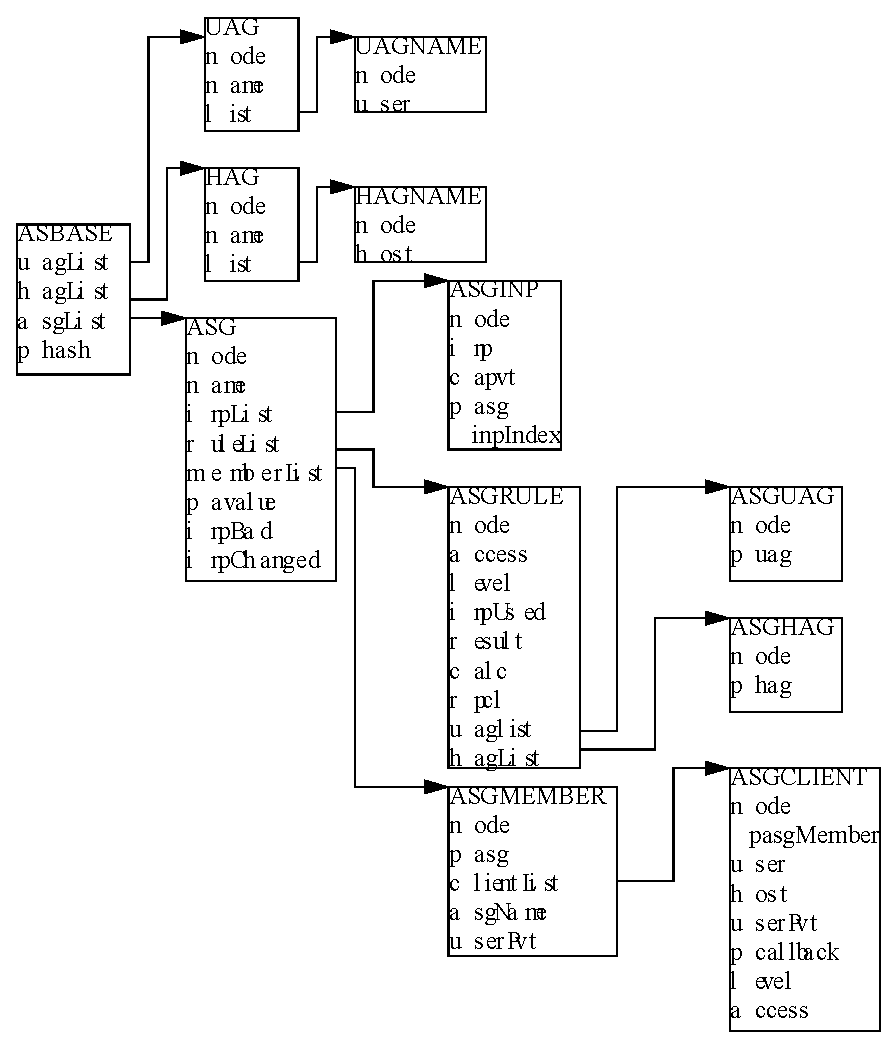
\includegraphics{accessSecurity_1}
\end{center}
